\CX{
\begin{onecolumnfigure}

\begin{fitwidth}{11.333\standardhexwidth}
\begin{tikzpicture}

\scriptsize

    \drawhexgrid{0}{0}{10}{3}

    \begin{athex}{1.00}{-0.50}
        \drawdashedcounter  {+0.00}{+1.00}{90}
        \drawaircraftcounter{+0.00}{+2.00}{90}{F-4}{}{}
        \drawaircraftcounter{+1.00}{+2.50}{90}{F-4}{}{}
        \drawdashedcounter  {+1.00}{+3.50}{90}
        \begin{scope}[shift={(135:0.3)},thick,->]
            \miniathex{0.00}{1.00}{\draw (90:0.1) -- (90:0.5);}
            \miniathex{1.00}{2.50}{\draw (90:0.1) -- (90:0.5);}
        \end{scope}
        \miniathex{+0.00}{+2.00}{\draw [thick,->] (30:0.35) -- (30:0.65);}
    \end{athex}

    \begin{athex}{2.50}{-0.25}
        \drawdashedcounter{+0.50}{+0.75}{60}
        \drawaircraftcounter{+1.00}{+1.50}{60}{F-4}{}{}
        \drawaircraftcounter{+2.00}{+2.00}{60}{F-4}{}{}
        \drawdashedcounter{+2.50}{+2.75}{60}
        \begin{scope}[shift={(105:0.3)},thick,->]
            \miniathex{+0.50}{+0.75}{\draw (60:0.05) -- (60:0.4);}
            \miniathex{+2.00}{+2.00}{\draw (60:0.05) -- (60:0.4);}
        \end{scope}
        \miniathex{+1.00}{+1.50}{\draw [thick,->] (30:0.35) -- (30:0.65);}
    \end{athex}
    
    \begin{athex}{5.00}{-0.50}
        \drawdashedcounter  {+0.50}{+0.75}{60}
        \drawaircraftcounter{+1.00}{+1.50}{60}{F-4}{}{}
        \drawaircraftcounter{+2.00}{+2.00}{60}{F-4}{}{}
        \drawdashedcounter  {+2.50}{+2.75}{60}
        \begin{scope}[shift={(105:0.3)},thick,->]
            \miniathex{+0.50}{+0.75}{\draw (60:0.05) -- (60:0.4);}
            \miniathex{+2.00}{+2.00}{\draw (60:0.05) -- (60:0.4);}
        \end{scope}
        \miniathex{+1.00}{+1.50}{\draw [thick,->] (30:0.35) -- (30:0.65);}
        \begin{scope}[shift={(315:0.5)},anchor=west]
            \miniathex{+0.50}{+0.75}{\draw node {start position};}
            \miniathex{+1.00}{+1.50}{\draw node {preparatory HFP};}
            \miniathex{+2.00}{+2.00}{\draw node {roll execution};}
            \miniathex{+2.50}{+2.75}{\draw node {next HFP};}
        \end{scope}
    \end{athex}

\end{tikzpicture}
\end{fitwidth}

\figurecaption{figure:displacement-roll-maneuvers}{Displacement Roll Maneuvers}

\end{onecolumnfigure}

}{

\begin{twocolumnfigure}

\begin{fitheight}{5.2\standardhexwidth}
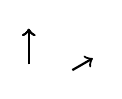
\begin{tikzpicture}
    \setfiguresize{-2.6}{-2.6}{+2.6}{+2.6}
    \begin{scope}
        \drawevenhexgrid{-2}{-2}{5}{5}
        \drawdashedcounter{+0.00}{-2.00}{0}
        \drawdashedcounter{+0.00}{-1.00}{0}
        \drawaircraftcounter{+0.00}{+0.00}{90}{F-4}{}{}
        \drawaircraftcounter{+1.00}{+0.50}{90}{F-4}{}{}
        \drawdashedcounter{+1.00}{+1.50}{0}
        \begin{scope}[shift={(-0.25,+0.25)},thick,->]
            \miniathex{+0.00}{-2.00}{\draw (90:0.0) -- (90:0.45);}
            \miniathex{+0.00}{-1.00}{\draw (90:0.0) -- (90:0.45);}
            \miniathex{+1.00}{+0.50}{\draw (90:0.0) -- (90:0.45);}
        \end{scope}
        \miniathex{+0.00}{+0.00}{\draw [thick,->] (30:0.35) -- (30:0.65);}
     \end{scope}
\end{tikzpicture}
\end{fitheight}
\hfil
\begin{fitheight}{5.2\standardhexwidth}
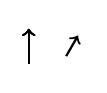
\begin{tikzpicture}
    \setfiguresize{-2.6}{-2.6}{+2.6}{+2.6}
    \begin{scope}[rotate=90]
        \drawevenhexgrid{-2}{-2}{5}{5}
        \drawdashedcounter{-2.00}{+0.00}{0}
        \drawdashedcounter{-1.00}{+0.00}{0}
        \drawaircraftcounter[90]{+0.00}{+0.00}{0}{F-4}{}{}
        \drawaircraftcounter[90]{+1.00}{-0.50}{0}{F-4}{}{}
        \drawdashedcounter{+2.00}{-0.50}{0}
        \begin{scope}[shift={(+0.20,+0.30)},thick,->]
            \miniathex{-2.00}{+0.00}{\draw (0:0.0) -- (0:0.45);}
            \miniathex{-1.00}{+0.00}{\draw (0:0.0) -- (0:0.45);}
            \miniathex{+1.00}{-0.50}{\draw (0:0.0) -- (0:0.45);}
        \end{scope}
        \miniathex{+0.00}{+0.00}{\draw [thick,->] (330:0.35) -- (330:0.65);}
        %\begin{scope}[shift={(+0.50,+0.75)},anchor=east]
        %    \miniathex{-2.00}{+0.00}{\draw node {\minitable{r}{preparatory\\ HFP}};}
        %    \miniathex{-1.00}{+0.00}{\draw node {\minitable{r}{preparatory\\ HFP}};}
        %    \miniathex{+0.00}{-0.50}{\draw node {\minitable{r}{roll\\ execution}};}
        %    \miniathex{+1.00}{-0.50}{\draw node {\minitable{r}{next\\ HFP}};}
        %\end{scope}
    \end{scope}
\end{tikzpicture}
\end{fitheight}
\hfil
\begin{fitheight}{5.2\standardhexwidth}
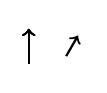
\begin{tikzpicture}
    \setfiguresize{-2.6}{-2.6}{+2.6}{+2.6}
    \begin{scope}[rotate=90]
        \drawoddhexgrid{-2}{-1.5}{5}{5}
        \drawdashedcounter{-2.00}{+0.00}{0}
        \drawdashedcounter{-1.00}{+0.00}{0}
        \drawaircraftcounter[90]{+0.00}{+0.00}{0}{F-4}{}{}
        \drawaircraftcounter[90]{+1.00}{-0.50}{0}{F-4}{}{}
        \drawdashedcounter{+2.00}{-0.50}{0}
        \begin{scope}[shift={(+0.20,+0.30)},thick,->]
            \miniathex{-2.00}{+0.00}{\draw (0:0.0) -- (0:0.45);}
            \miniathex{-1.00}{+0.00}{\draw (0:0.0) -- (0:0.45);}
            \miniathex{+1.00}{-0.50}{\draw (0:0.0) -- (0:0.45);}
        \end{scope}
        \miniathex{+0.00}{+0.00}{\draw [thick,->] (330:0.35) -- (330:0.65);}
    \end{scope}
\end{tikzpicture}
\end{fitheight}

\figurecaption{figure:displacement-roll-maneuvers}{Displacement rolls to the right, each preceded by two preparatory HFPs and followed by another HFP. The execution of the roll is indicated by the counter images with solid borders. The number of preparatory FPs required depends on the aircraft speed and other factors. The execution of a displacement roll is identical to that of a slide, although other aspects are different.}

\end{twocolumnfigure}
}
